\documentclass[
  letterpaper,
  twocolumn,
  9pt,
  journal,
  final]{IEEEtran}

\usepackage[spanish,es-tabla]{babel}
\usepackage[utf8]{inputenc}
\usepackage{amsfonts}
\usepackage{amsmath}
\usepackage{amssymb}
\usepackage{amsxtra}
\usepackage{mathrsfs}
\usepackage{array}
\usepackage{tikz}
\usepackage{cite}
\usepackage{varioref}
\usepackage{float}
\usepackage{color}
\usepackage{colortbl}
\usepackage{enumerate}
\usepackage{rotating}
\usepackage{subcaption}
\usepackage{hyperref}
\usepackage{listings}
\usepackage{lipsum}
%\usepackage{flushend}
\usepackage{graphicx}
\usepackage{xcolor}
\hypersetup{
    colorlinks,
    linkcolor={red!50!black},
    citecolor={blue!50!black},
    urlcolor={blue!80!black}
}

\usepackage{lipsum}

\title{Tarea 4 - Procesamiento Digital de Imágenes}
\author{\textbf{Autor:} Pablo Yáñez Santibáñez - pablo.yanez@uai.cl}
%\author{\IEEEauthorblockN{Pablo Yáñez S.} - pablo.yanez@uai.cl}

% Levels to show in table of contents:
% \setcounter{tocdepth}{-1} % only parts
% \setcounter{tocdepth}{0}  % only parts and chapters
% \setcounter{tocdepth}{1}  % part,chapters,sections
\setcounter{tocdepth}{2}  % part,chapters,sections, subsections
% \setcounter{tocdepth}{3}  % part,chapters,sections, subsections,subsubsections
% \setcounter{tocdepth}{4}  % part,chapters,sections, subsections,subsubsections and paragraphs
% \setcounter{tocdepth}{5}  % part,chapters,sections, subsections, subsubsections, paragraphs and subparagraphs.

\begin{document}
\bstctlcite{IEEEexample:BSTcontrol}
\maketitle

% \begin{abstract}
% We propose \lipsum[1]
% \end{abstract}

\tableofcontents

% \listoffigures

% \listoftables

%%%%%%%%%%%%%%%%%%%%%%%%%%%%%%%%%%%%%%%%%%%%%%%%%%%%%%%%%%%%%%%%%%%%%%%%%%%%%%%%

\section{Introducción}

Para el desarrollo de este trabajo se descarga una imagen de Los Dientes de Navarino (Puerto Williams) del sitio \href{https://www.flickr.com/photos/whitewizard/7062826349/in/album-72157629780861323/}{Flickr}. Esta imagen es usada para las distintas actividades que se describen en este documento.

\begin{figure}[h!]
	\centering
	% 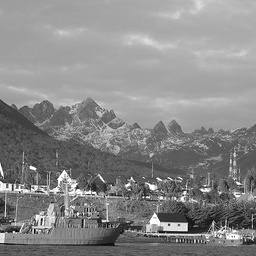
\includegraphics[width=0.6\linewidth, trim={0cm 0cm 0cm 5cm}, clip]{outs/gaussiano/img.jpg}
	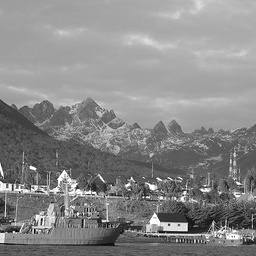
\includegraphics[width=0.4\linewidth, trim={0cm 0cm 0cm 0cm}, clip]{outs/gaussiano/img.jpg}
	\caption{Dientes de Navarino.}
	\label{dientes}
\end{figure}

\section{Marco Teórico}

\subsection{Imagen}

Se puede describir una imagen $g(x,y)$ como una composición de una imagen ideal $f(x,y)$ degradada por un proceso $h(x,y)$ más una componente de ruido $\eta(x,y)$.

\begin{align}
  g(x,y) = h(x, y) * f(x,y) + \eta(x,y)
\end{align}

Luego se tiene como objetivo poder recuperar la información de la imagen original a traves de un proceso de restauración. La Figura \ref{restauracion} presenta un diagrama del proceso general.

\begin{figure}[h!]
	\centering
	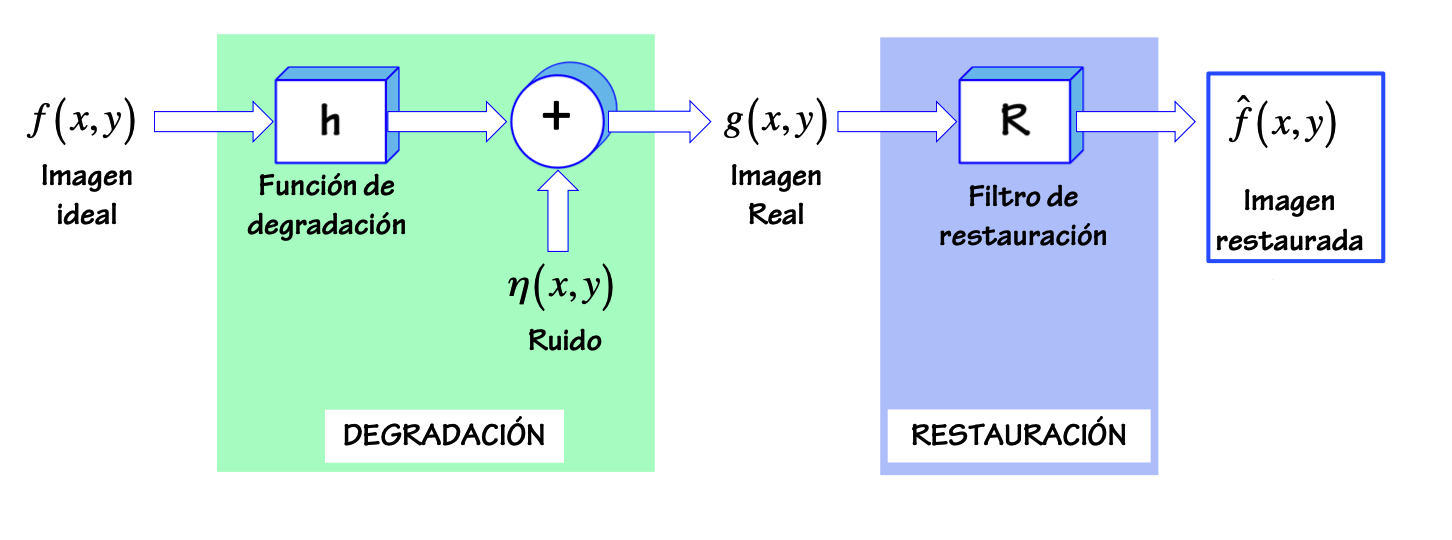
\includegraphics[width=0.8\linewidth, trim={0cm 0cm 1cm 0cmm}, clip]{other/restauracion.png}
	\caption{Diagrama proceso restauración \cite{carrasco3}.}
	\label{restauracion}
\end{figure}


\subsection{Ruido}

El las señales el ruido corresponde a una señal no deseada que se mezcla con la señal util. En el caso de las imagenes el ruido hace que un pixel de una imagen tome un valor que no corresponde al original. El ruido se puede catalogar de acuerdo a su naturaleza.

\subsubsection{Ruido Gaussiano:}
El ruido gaussiano se describe como una variable que sigue una distribución normal. En el caso de las imagenes, el ruido gaussiano se modela como un ruido aditivo, lo que significa que cada pixel es la suma de la información original más un una componente de ruido con distribución normal. La Figura \ref{gauss} muestra el efecto de aplicar ruido gaussiano a la imagen original con distintos valores de $\sigma$

\begin{figure}[!tbh]
  \centering
  \begin{subfigure}[b]{.32\linewidth}
    \includegraphics[width=\linewidth]{outs/gaussiano/noisy_005.jpg}
    \caption{$\sigma=0.05$}\label{gauss_0.05}
  \end{subfigure}
  \begin{subfigure}[b]{.32\linewidth}
    \includegraphics[width=\linewidth]{outs/gaussiano/noisy_010.jpg}
    \caption{$\sigma=0.1$}\label{gauss_0.10}
  \end{subfigure}
  \begin{subfigure}[b]{.32\linewidth}
    \includegraphics[width=\linewidth]{outs/gaussiano/noisy_050.jpg}
    \caption{$\sigma=0.5$}\label{lata_gauss_0.50}
  \end{subfigure}
  \caption{Imagen con ruido gaussiano.}
  \label{gauss}
\end{figure}

\subsubsection{Ruido Impulsional:}
El ruido impulsional corresponde a impulsos que contaminan la señal util con valores altos o bajos. En las imagenes el ruido impulsional hace que un pixel tome valores 0 o 255. Generalmente el ruido sigue una distribución normal. En el caso de que el ruido solo contamine con valores 0 se conoce como ruido pimienta, mientras que si contamina con valores 255 toma el nombre de ruido sal. La Figura \ref{impulsional} muestra ejemplos de ruido impulsional aplicado a la imagen original.

\begin{figure}[!tbh]
  \centering
  \begin{subfigure}[b]{.32\linewidth}
    \includegraphics[width=\linewidth]{outs/pimienta/noisy.jpg}
    \caption{Pimienta}\label{pimienta}
  \end{subfigure}
  \begin{subfigure}[b]{.32\linewidth}
    \includegraphics[width=\linewidth]{outs/sal/noisy.jpg}
    \caption{Sal}\label{sal}
  \end{subfigure}
  \begin{subfigure}[b]{.32\linewidth}
    \includegraphics[width=\linewidth]{outs/sal/noisy_sp.jpg}
    \caption{Sal y pimienta}\label{sal_pimienta}
  \end{subfigure}
  \caption{Imagen con ruido impulsional.}
  \label{impulsional}
\end{figure}

\subsubsection{Ruido Uniforme:}

El ruido uniforme hace que una señal pueda tomar un valor en un intervalo con una probabilidad constante. En el caso de una imagen, el ruido uniforme hace que la probabilidad de tomar cualquier valor de gris en un intervalo es constante. Ejemplos de aplicar ruido uniforme a la imagen original se presentan en la Figura \ref{uniforme}.

\begin{figure}[!tbh]
  \centering
  \begin{subfigure}[b]{.32\linewidth}
    \includegraphics[width=\linewidth]{outs/uniforme/noisy_b040.jpg}
    \caption{$a=10, b=40$}\label{uni1}
  \end{subfigure}
  \begin{subfigure}[b]{.32\linewidth}
    \includegraphics[width=\linewidth]{outs/uniforme/noisy_b060.jpg}
    \caption{$a=10, b=60$}\label{uni1}
  \end{subfigure}
  \begin{subfigure}[b]{.32\linewidth}
    \includegraphics[width=\linewidth]{outs/uniforme/noisy_b150.jpg}
    \caption{$a=10, b=150$}\label{uni1}
  \end{subfigure}
  \caption{Imagen con ruido uniforme.}
  \label{uniforme}
\end{figure}

\subsection{Modelos de Degradación}

\subsubsection{Turbulencia}

El modelo de turbulencia esta dado por (\ref{turb}). A través de la Transformada de Fourier el fenomeno de turbulencia puede modelarse como una multiplicación en el dominio de la frecuencia, donde el modelo de degradación esta dado por (\ref{turb_fourier}). La Figura \ref{turb} presenta tres ejemplos de aplicar la función de degradación a la imagen de la Figura \ref{dientes}.

\begin{align}
  g(x, y) &= h(x,y) * f(x,y) \label{turb} \\
  H(u,v) &= e ^ {-k (u^2 + v^2) \frac{5}{6}} \label{turb_fourier}
\end{align}

\begin{figure}[!tbh]
  \centering
  \begin{subfigure}[b]{.32\linewidth}
    \includegraphics[width=\linewidth]{outs/degradacion/turb_01.jpg}
    \caption{$k=0.001$}\label{turb1}
  \end{subfigure}
  \begin{subfigure}[b]{.32\linewidth}
    \includegraphics[width=\linewidth]{outs/degradacion/turb_05.jpg}
    \caption{$k=0.005$}\label{turb5}
  \end{subfigure}
  \begin{subfigure}[b]{.32\linewidth}
    \includegraphics[width=\linewidth]{outs/degradacion/turb_05.jpg}
    \caption{$k=0.009$}\label{turb9}
  \end{subfigure}
  \caption{Ejemplo de Turbulencia.}
  \label{turb}
\end{figure}

\subsubsection{Movimiento Lineal}

El modelo de movimiento lineal replica el efecto de movimiento que ocurre cuando el objeto enfocado o el fotografo se mueve. El modelo de degradación en el dominio de la frecuencia se describe se segun (\ref{mov_lineal}), donde los parámetros $a$, $b$ y $T$ son escalares. La Figura \ref{Movimiento_Lineal} presenta unos ejemplos de aplicar la degradación de movimiento lineal variando los parámetros de la función de degradación.

\begin{align}
  H(u,v) = T e^{-i\pi (ua + vb)} sinc( \pi (ua + vb)) \label{mov_lineal}
\end{align}

\begin{figure}[!tbh]
  \centering
  \begin{subfigure}[b]{.32\linewidth}
    \includegraphics[width=\linewidth]{outs/degradacion/mov_3_0_1.jpg}
    \caption{$a=3, b=0, T=1$}\label{mov1}
  \end{subfigure}
  \begin{subfigure}[b]{.32\linewidth}
    \includegraphics[width=\linewidth]{outs/degradacion/mov_0_3_1.jpg}
    \caption{$a=0, b=3, T=1$}\label{mov2}
  \end{subfigure}
  \begin{subfigure}[b]{.32\linewidth}
    \includegraphics[width=\linewidth]{outs/degradacion/mov_3_3_1.jpg}
    \caption{$a=3, b=3, T=1$}\label{mov3}
  \end{subfigure}
  \caption{Ejemplo de Movimiento Lineal.}
  \label{Movimiento_Lineal}
\end{figure}

\subsection{Filtros en el dominio espacial}

A continuación se describen los filtros en el dominio del espacio utilizados en este trabajo.

\subsubsection{Filtro Gaussiano}
Corresponde un filtro de la familia de filtros lineales. El filtro utiliza una máscara con distribución gaussiana normalizada.

\subsubsection{Filtro Max-Min}
Este filto de la familia de filtros estadisticos. El filtro reemplaza el valor central de la máscara por el valor mínimo o máximo de las misma máscara.

\subsubsection{Filtro Mediana Adaptivo}


\section{Desarrollo}

\subsection{Ruido Gaussiano}

\begin{figure}[!tbh]
  \centering
  \begin{subfigure}[b]{.32\linewidth}
    \includegraphics[width=\linewidth]{outs/gaussiano/noisy_005.jpg}
    \caption{$\sigma=0.05$}\label{gauss_0.05}
  \end{subfigure}
  \begin{subfigure}[b]{.32\linewidth}
    \includegraphics[width=\linewidth]{outs/gaussiano/noisy_010.jpg}
    \caption{$\sigma=0.1$}\label{gauss_0.10}
  \end{subfigure}
  \begin{subfigure}[b]{.32\linewidth}
    \includegraphics[width=\linewidth]{outs/gaussiano/noisy_050.jpg}
    \caption{$\sigma=0.5$}\label{lata_gauss_0.50}
  \end{subfigure}
  \caption{Imagen con ruido gaussiano.}
  \label{gauss}
\end{figure}

\subsection{Ruido Sal}

\subsection{Ruido Pimienta}

\subsection{Ruido Uniforme}




%%%%%%%%%%%%%%%%%%%%%%%%%%%%%%%%%%%%%%%%%%%%%%%%%%%%%%%%%%%%%%%%%%%%%%%%%%%%%%%%
% Bibliography
\nocite{*}
\bibliographystyle{IEEEtran}
\bibliography{bibliography}


\end{document}
